\documentclass[10pt,a4paper]{article}
\usepackage[utf8]{inputenc}
\usepackage[english]{babel}
\usepackage{amsmath}
\usepackage{amsfonts}
\usepackage{amssymb}
\usepackage{makeidx}
\usepackage{graphicx}
\usepackage{lmodern}
\usepackage{graphics}
\usepackage{caption}
\usepackage{subcaption}
\usepackage{listings}

\usepackage{color} %red, green, blue, yellow, cyan, magenta, black, white
\definecolor{mygreen}{RGB}{28,172,0} % color values Red, Green, Blue
\definecolor{mylilas}{RGB}{170,55,241}
\definecolor{mygray}{rgb}{0.5,0.5,0.5}
\definecolor{mymauve}{rgb}{0.58,0,0.82}
\definecolor{myblue}{rgb}{0.33,0.33,0.99}



\title{Algoritmos y Programación II\\
Trabajo Práctico 0}
\author{Carlos Germán Carreño Romano, Sebastián Sampayo, Rodrigo Bourbon}
\begin{document}
\maketitle
\tableofcontents

\section{Introducción}


\subsection{Radio definida por software (SDR)}

El concepto de Radio Definida por Software se le atribuye a Joseph Mitola, 1990. Se refiere a un dispositivo que permite reducir al mínimo el hardware necesario para la recepción de señales de radio. Dicho equipo captura la señal analógica (ya sea mediante un cable o una antena), la digitaliza (mediante un conversor A/D) para luego realizar por software toda la etapa de procesamiento de señal requerido en la decodificación. Esto ha logrado que la recepción de cierto rango de telecomunicaciones sea mucho más accesible en términos económicos y prácticos (ya que el mismo dispositivo físico se puede utilizar para distintos fines con solo re-programar el software). Un ejemplo de este dispositivo se puede ver a continuación:

\begin{figure}
\begin{centering}
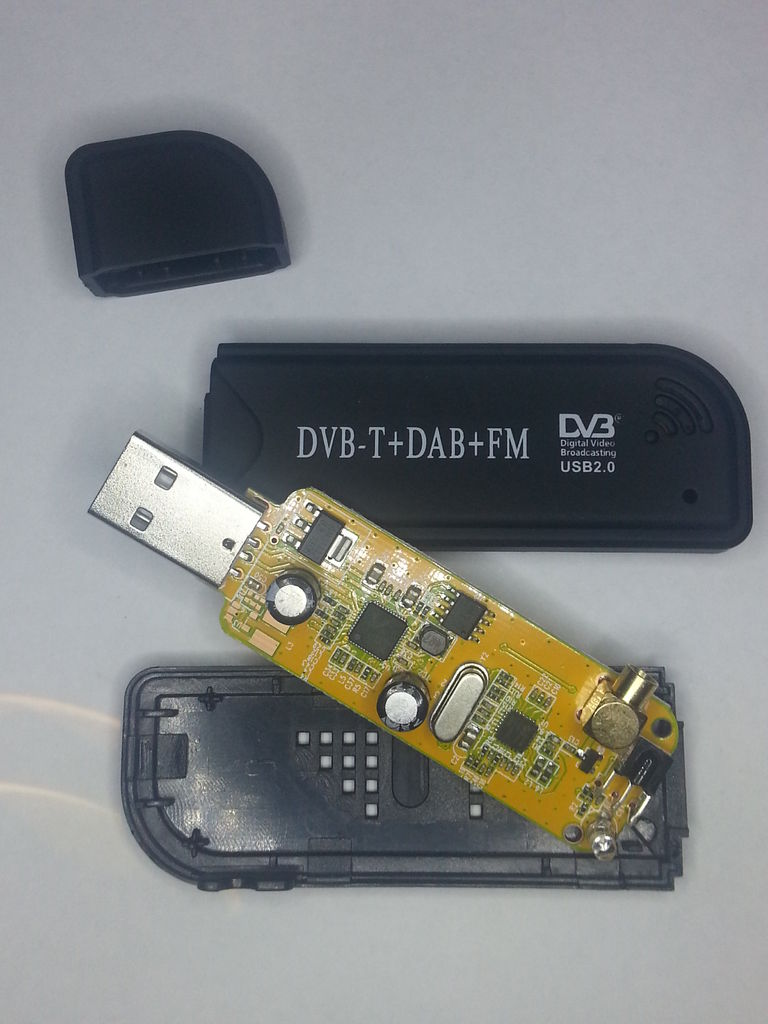
\includegraphics[width=0.5\textwidth]{Imagenes/SDR.jpg}
\par\end{centering}
\caption{Sintonizador de radio digital.}
\end{figure}



\subsection{Transmisión de TV por cable}

En telecomunicaciones, la televisión analógica se transmite mediante
el método de la Multiplexión por División en Frecuencia (FDM). Esta
técnica consiste en transmitir varias señales simultáneamente modulando
cada una con una portadora diferente, en el rango de VHF/UHF, de forma
tal que los anchos de banda de cada señal no se superpongan significativamente.
El canal destinado para la transmisión de una emisora tiene un ancho
de banda de aproximadamente 6 Mhz, donde los 5.45 Mhz más bajos corresponden
al espectro de la señal de video y los últimos 0.55Mhz (aproximadamente)
se reservan para el espectro de la señal de audio. Este modelo de
comunicación se puede ver representado en la figura 2:

\begin{figure}
\begin{centering}
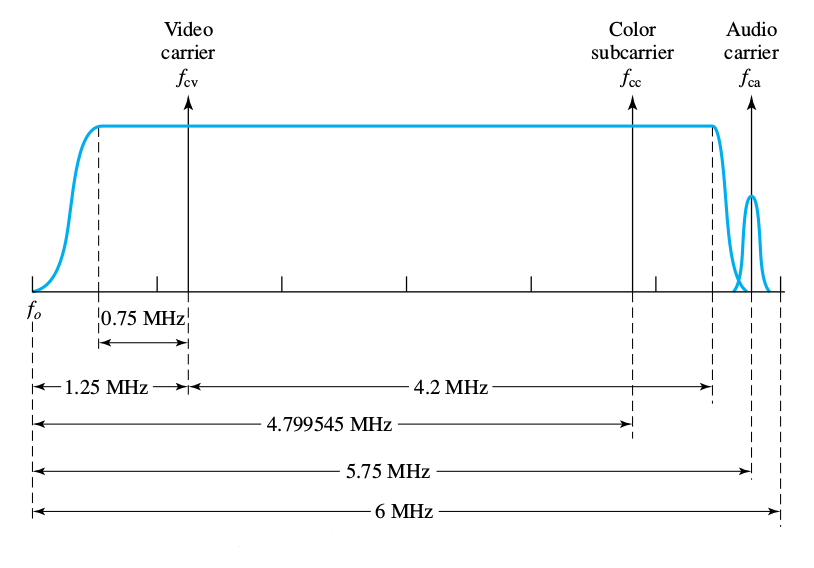
\includegraphics[width=0.5\textwidth]{Imagenes/TV_Spectrum.png}
\par\end{centering}
\caption{Señal de TV transmitida.}
\end{figure}



\subsection{Aplicación del Trabajo Práctico}

Sabiendo que el audio de la televisión está modulado en frecuencia
(FM), si se toma la porción del canal adecuada es posible demodular
dicha señal y escuchar algún canal de televisión.

En este caso particular, el SDR se utilizó para capturar un ancho
de banda de 2.4Mhz y centrado en 181.238 Mhz. A través del aplicativo
desarrollado se pudo escuchar efectivamente el programa emitido.


\section{Desarrollo}
\subsection{Pseudocódigo}
Las siguientes notas sirvieron como borrador del pseudocódigo para alinear ideas y codificar las funciones principales.\\
\begin{verbatim}
- i := 0
- j := 0
- buffer1 := 0
- buffer2 := 0

( -- Condiciones Iniciales Nulas -- )
- x_prev := 0

- Mientras haya complejos en la entrada
	( -- Promediar 11 elementos -- )
	- buffer1 := buffer1 + complejo a la entrada
	- Si i < 10
		- i := i + 1
		- Continuar con el ciclo
	- x := buffer1 / 11
	- buffer1 := 0
	- i := 0

	( -- Obtener la derivada de la fase -- )
	- aux := x * conjugar(x_prev)
	- aux := fase(aux)

	( -- Avanzar una muestra -- )
	- x_prev := x

	( -- Promediar 4 elementos -- )
	- buffer2 := buffer2 + aux
	- Si j < 3
		- j := j + 1
		- Continuar con el ciclo
	- resultado := buffer2 / 4
	- buffer2 := 0
	- j := 0
	
	( -- Imprimir en el formato especificado -- )
	- resultado := (resultado + pi)*255/2pi 

\end{verbatim}
\subsection{Implementación}
Para implementar el proceso propuesto en la especificación del presente trabajo, se descubrió que la cascada de los bloques "Promediador móvil de N elementos" seguido de "Decimador de N elementos", es totalmente equivalente a un único bloque en el cual se tomen N elementos y cuya salida sea el promedio de dichos N elementos. A continuación se toman los siguientes N elementos y la nueva salida es el promedio de estos últimos N elementos, y así sucesivamente.\\

 Consecuentemente, se optó por implementar este último algoritmo a fin de simplificar el código del trabajo. En concreto se utilizaron sentencias básicas de control de flujo (\'while\', \'if\', \'continue\'). Esto se puede ver en el siguiente extracto del \'main\':

\begin{verbatim}
(...)
//Mientras haya complejos en la entrada
  while (*iss >> input_complex)
  {
    // ( -- Promediar 11 elementos -- )
    buffer1 += input_complex;
    if (i < DECIMATOR1_SIZE-1)
    {
      i++;
      continue;
    }
    x = buffer1/DECIMATOR1_SIZE;
    buffer1 = 0;
    i = 0;
(...)
  }
\end{verbatim}
La idea es ir acumulando en un \'buffer\' la suma de los complejos a la entrada (\'input\_complex\'), hasta que hayan pasado 11 elementos (parametrizado por \'DECIMATOR1\_SIZE\'). En dicho momento la condición del \'if\' no se cumple y entonces se divide al valor del \'buffer\' por 11 para obtener la salida del bloque. Luego se vacía el buffer y se reinicializa la cuenta.\\



\subsection{Estándar de estilo}
Adoptamos la convención de code styling de Google para C++, salvando las siguientes excepciones:\\
\begin{itemize}
\item streams: utilizamos flujos de entrada y salida
\item sobrecarga de operadores
\item 

Para notación de archivos, variables, clases, tipos de datos y variables globales nos seguimos de la regla detallada en:
\begin{verbatim}
https://google-styleguide.googlecode.com/svn/trunk/cppguide.html#Naming
\end{verbatim}
\end{itemize}

\section{Compilación}
Para compilar los códigos fuentes utilizamos el compilador g++, de la Free Software Foundation \footnote{www.fsf.org}, con la opción -Wall, que activa cualquier tipo de advertencia además de los errores de compilación. \\
El proceso de compilación se realiza con el comando \begin{verbatim}
make
\end{verbatim}
que ejecuta el archivo Makefile, donde se detalla el árbol de archivos del programa, la compilación de cada código objeto por separado, y algunos comentarios. El archivo Makefile se detalla a continuación:\\
\begin{verbatim}
CC      = g++
CCFLAGS  = -g -Wall -pedantic
LDFLAGS  =
OBJS = main.o complex.o cmdline.o
PROGRAM_NAME = tp0

all: tp0
#	@/bin/true

tp0: $(OBJS)
	$(CC) $(LDFLAGS) $(OBJS) -o $(PROGRAM_NAME)

main.o: main.cc complex.h cmdline.h
	$(CC) $(CCFLAGS) -c main.cc

complex.o: complex.cc complex.h
	$(CC) $(CCFLAGS) -c complex.cc
	
cmdline.o: cmdline.cc cmdline.h
	$(CC) $(CCFLAGS) -c cmdline.cc


clean:
	rm *.o
\end{verbatim}
\subsection{Opciones del programa}
Los argumentos posibles para pasarle a la línea de comandos del programa son los siguientes (el orden enq ue aparezcan no tiene importancia):
\begin{itemize}
\item  Ingreso de datos: es un argumento obligatorio y se indica en su forma corta mediante "-i" y en su forma larga mediante "--input". Se le debe pasar siempre una opción que debe ser la ruta de un archivo del cual queramos leer o bien la opción por defecto "-" que utiliza el flujo de entrada estándar.

\item  salida de datos: es un argumento obligatorio y se indica en su forma corta mediante "-o" y en su forma larga mediante "--output". Se le debe pasar siempre una opción que debe ser la ruta de un archivo en el cual queramos imprimir o bien la opción por defecto "-" que utiliza el flujo de salida estándar.

\item  Formato de ingreso/salida de datos: es un argumento opcional, siendo la opción por defecto la de modo texto y se indica en su forma corta mediante "-f" y en su forma larga mediante "--format". Las opciones que recibe este argumento son:

	- Fornato texto: "txt".\\
	- Formato U8: "U8".\\

Ambas opciones de formato analizan la entrada y producen una salida de acuerdo a lo establecido en el enunciado del trabajo. Para caracterizarlas, en el programa se definió un tipo enumerativo con las opciones y un atributo privado de este tipo en la clase "Complex" para al momento de crear un objeto de la clase pasarle como argumento el formato. Este atributo es útil al momento de ejecutar la lectura de la entrada. Esto se realizó sobreescribiendo los flujos de entrada y salida (">>" y "<<" respectivamente) y declarando un método privado particular para cada formato (se definieron como privados porque son relativos a la impementación). Los métodos de los flujos llaman al método correspondiente mediante una selección con la sentencia "switch", que evalúa el atributo de formato del complejo en el que se está leyendo.
La salida resultante es un valor que también depende del formato elegido, por lo tanto se codificó una función para cada caso  y se seleciona la que corresponde mediante un puntero de arreglos a función.
Esta estructura del programa nos proporciona escalabilidad y mantenibilidad, ya que se codificaron módulos dedicados para cada operación y si se agrega una nueva opción solo se debe codificar otro módulo, o si falla alguno la reaparación es específica de ese módulo.
Para la compilación

\end{itemize}

\section{Ejecución}
En los siguientes casos de prueba requeridos en el enunciado, se ejecutó el programa desarrollado en una consola linux. Se muestra a continuación las imágenes con las corridas del programa para los distintos casos.\\
\subsection{Casos de prueba}
\subsection{Caso 1}
\begin{center}
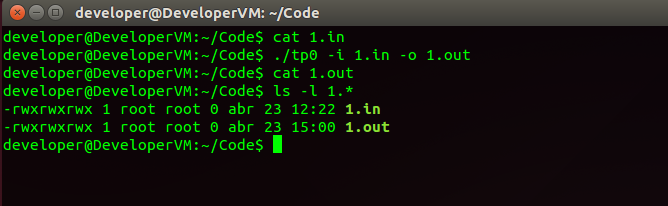
\includegraphics[scale=0.4]{Imagenes/Caso1.png} 
\end{center}
\subsection{Caso 2}
\begin{center}
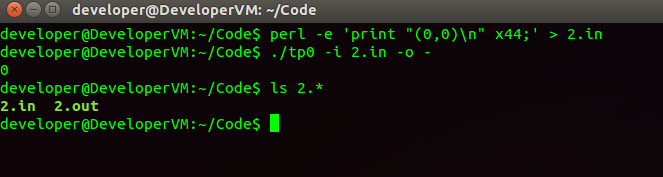
\includegraphics[scale=0.4]{Imagenes/Caso2.png} 
\end{center}
\subsection{Caso 3}
\begin{center}
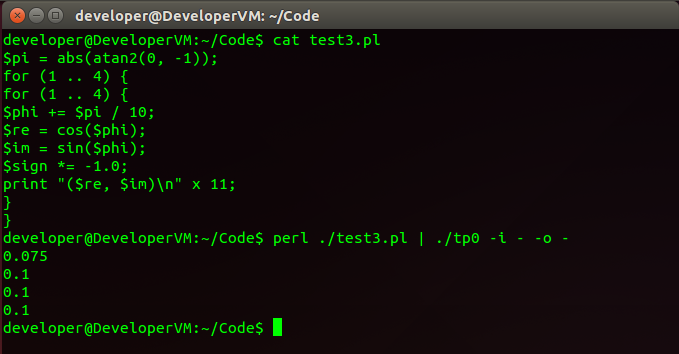
\includegraphics[scale=0.4]{Imagenes/Caso3.png} 
\end{center}
\subsection{Caso 4}
\begin{center}
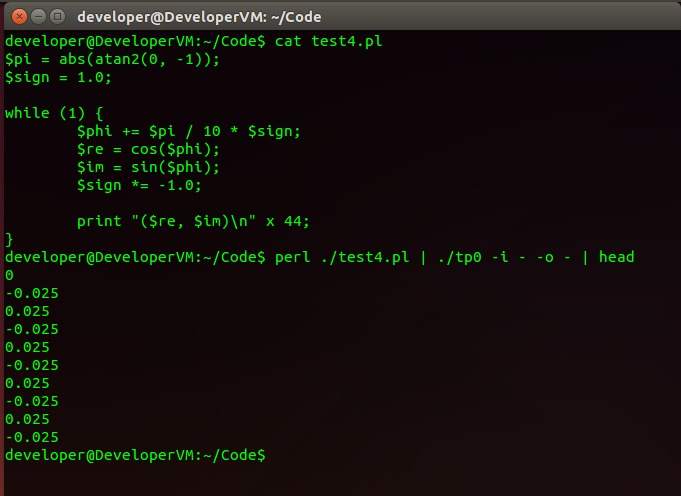
\includegraphics[scale=0.4]{Imagenes/Caso4.png} 
\end{center}
\subsection{Caso 5}
\begin{center}
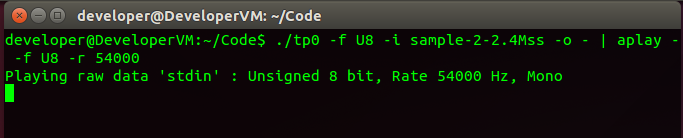
\includegraphics[scale=0.4]{Imagenes/Caso5.png} 
\end{center}
\section{Códigos}
A continuación se adjuntan los códigos fuente de todos los archivos utilizados en este proyecto. Para tener una referencia, el árbol de archivos descripto en el makefile tiene una referencia gráfica en la siguiente sección.\\
\subsection{Estructura de archivos}
\begin{center}
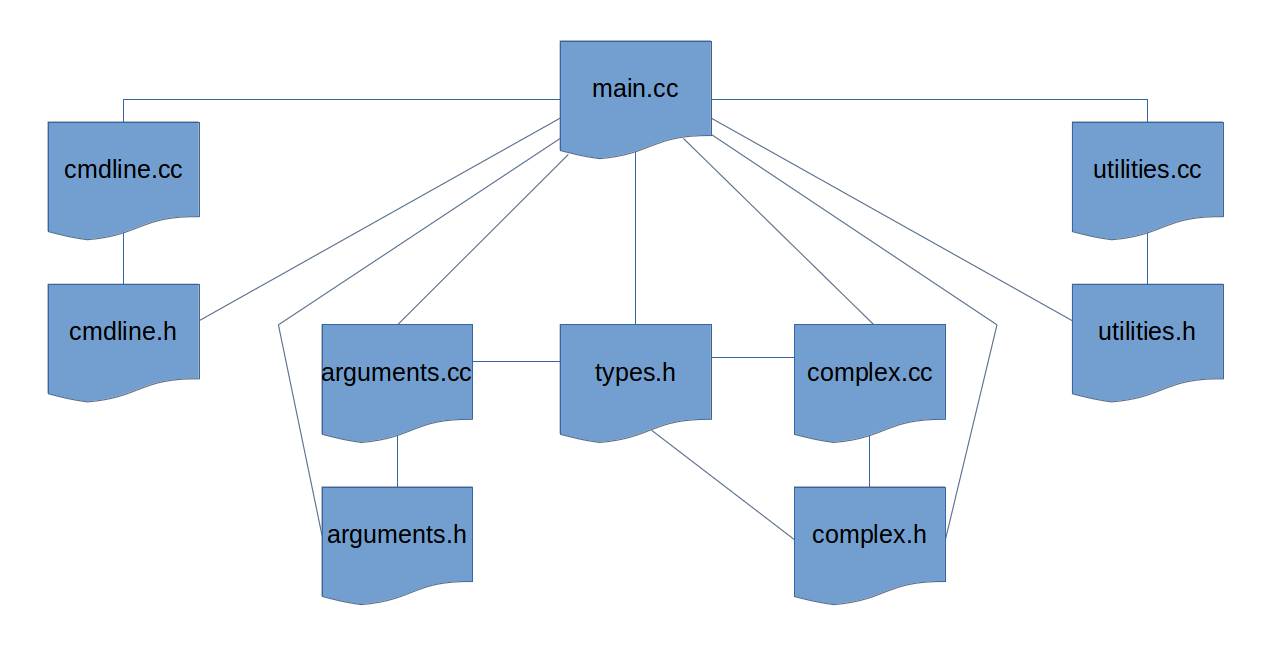
\includegraphics[scale=0.25]{Imagenes/Jerarquia_de_archivos.png} 
\end{center}

\lstset{language=C++,%
    basicstyle=\color{red},
    breaklines=true,%
    morekeywords={matlab2tikz},
    keywordstyle=\color{blue},%
    morekeywords=[2]{1}, keywordstyle=[2]{\color{green}},
    identifierstyle=\color{black},%
    stringstyle=\color{mygreen},
    commentstyle=\color{mygray},%
    showstringspaces=false,%without this there will be a symbol in the places where there is a space
    numbers=left,%
    numberstyle={\tiny \color{mygray}},% size of the numbers
    numbersep=9pt, % this defines how far the numbers are from the text
    emph=[1]{for,end,break},emphstyle=[1]\color{blue}, %some words to emphasise
    emph=[2]{word1,word2}, emphstyle=[2]{style},    
}
\subsection*{main}
\lstinputlisting{Code/main.cc}
\subsubsection*{main.h}
\lstinputlisting{Code/main.h}
\subsubsection*{utilities.h}
\lstinputlisting{Code/utilities.h}
\lstinputlisting{Code/utilities.cc}
\subsection{Clase Complex}
\subsubsection*{complex.h}
\lstinputlisting{Code/complex.h}
\subsubsection*{complex.cc}
\lstinputlisting{Code/complex.cc}

\subsection{Clase cmdline}
\subsubsection*{cmdline.h}
\lstinputlisting{Code/cmdline.h}
\subsubsection*{cmdline.cc}
\lstinputlisting{Code/cmdline.cc}
\subsubsection*{arguments.h}
\lstinputlisting{Code/arguments.h}
\subsubsection*{arguments.cc}
\lstinputlisting{Code/arguments.cc}

\newpage
\section{Enunciado}
\end{document}